\documentclass{standalone}
\usepackage{tikz}
\usetikzlibrary{patterns, positioning}

\begin{document}
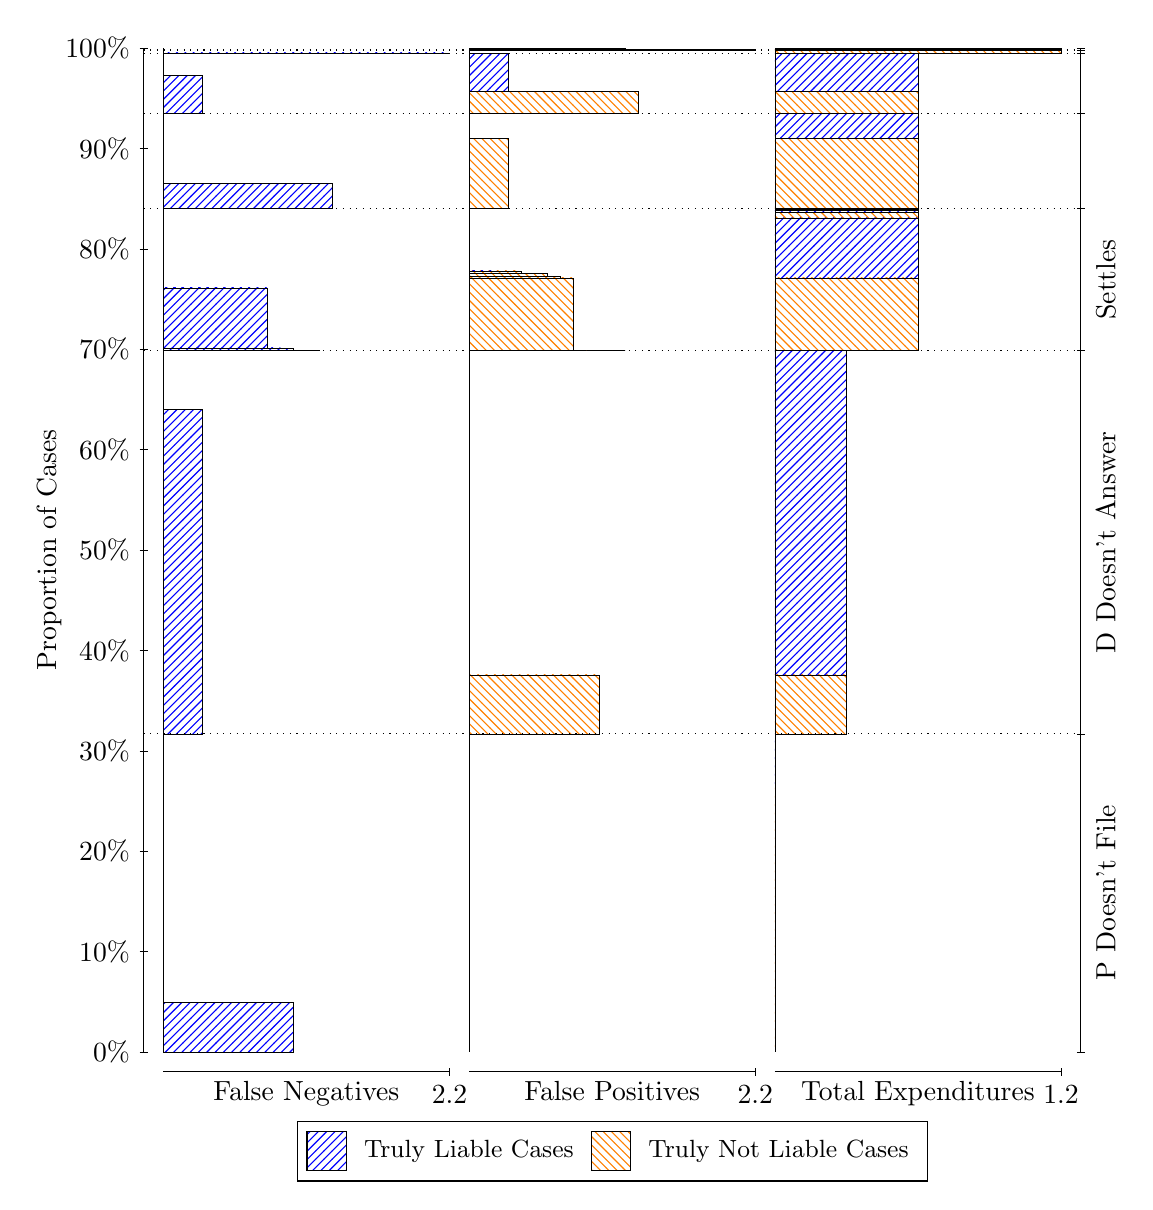
\begin{tikzpicture}
\draw[black, very thin] (1.5,1.75) -- (1.5,14.5);
\node[rotate=90, anchor=center] at (0.3, 8.125) {Proportion of Cases};
\draw[black, very thin] (1.45,1.75) -- (1.55,1.75);
\node[anchor=east] at (1.45, 1.75) {0\%};
\draw[black, very thin] (1.45,3.025) -- (1.55,3.025);
\node[anchor=east] at (1.45, 3.025) {10\%};
\draw[black, very thin] (1.45,4.3) -- (1.55,4.3);
\node[anchor=east] at (1.45, 4.3) {20\%};
\draw[black, very thin] (1.45,5.575) -- (1.55,5.575);
\node[anchor=east] at (1.45, 5.575) {30\%};
\draw[black, very thin] (1.45,6.85) -- (1.55,6.85);
\node[anchor=east] at (1.45, 6.85) {40\%};
\draw[black, very thin] (1.45,8.125) -- (1.55,8.125);
\node[anchor=east] at (1.45, 8.125) {50\%};
\draw[black, very thin] (1.45,9.4) -- (1.55,9.4);
\node[anchor=east] at (1.45, 9.4) {60\%};
\draw[black, very thin] (1.45,10.675) -- (1.55,10.675);
\node[anchor=east] at (1.45, 10.675) {70\%};
\draw[black, very thin] (1.45,11.95) -- (1.55,11.95);
\node[anchor=east] at (1.45, 11.95) {80\%};
\draw[black, very thin] (1.45,13.225) -- (1.55,13.225);
\node[anchor=east] at (1.45, 13.225) {90\%};
\draw[black, very thin] (1.45,14.5) -- (1.55,14.5);
\node[anchor=east] at (1.45, 14.5) {100\%};

\draw[black, very thin] (13.4,1.75) -- (13.4,14.5);
\draw[black, very thin] (13.35,1.75) -- (13.45,1.75);
\node[anchor=west] at (13.35, 1.75) {};
\draw[black, very thin] (13.35,5.7908) -- (13.45,5.7908);
\node[anchor=west] at (13.35, 5.7908) {};
\draw[black, very thin] (13.35,10.656) -- (13.45,10.656);
\node[anchor=west] at (13.35, 10.656) {};
\draw[black, very thin] (13.35,12.467) -- (13.45,12.467);
\node[anchor=west] at (13.35, 12.467) {};
\draw[black, very thin] (13.35,13.671) -- (13.45,13.671);
\node[anchor=west] at (13.35, 13.671) {};
\draw[black, very thin] (13.35,14.428) -- (13.45,14.428);
\node[anchor=west] at (13.35, 14.428) {};
\draw[black, very thin] (13.35,14.475) -- (13.45,14.475);
\node[anchor=west] at (13.35, 14.475) {};
\draw[black, very thin] (13.35,14.5) -- (13.45,14.5);
\node[anchor=west] at (13.35, 14.5) {};

\draw[black, very thin, pattern color=blue, pattern=north east lines] (1.75,1.75) rectangle (3.4015,2.3846);
\draw[black, very thin, pattern color=orange, pattern=north west lines] (1.75,2.3846) rectangle (1.75,5.7908);
\draw[black, very thin, pattern color=blue, pattern=north east lines] (1.75,5.7908) rectangle (2.2455,9.9078);
\draw[black, very thin, pattern color=orange, pattern=north west lines] (1.75,9.9078) rectangle (1.75,10.656);
\draw[black, very thin, pattern color=blue, pattern=north east lines] (1.75,10.656) rectangle (3.7318,10.663);
\draw[black, very thin, pattern color=blue, pattern=north east lines] (1.75,10.663) rectangle (3.5667,10.664);
\draw[black, very thin, pattern color=blue, pattern=north east lines] (1.75,10.664) rectangle (3.4015,10.681);
\draw[black, very thin, pattern color=blue, pattern=north east lines] (1.75,10.681) rectangle (3.2364,10.681);
\draw[black, very thin, pattern color=blue, pattern=north east lines] (1.75,10.681) rectangle (3.2364,10.691);
\draw[black, very thin, pattern color=blue, pattern=north east lines] (1.75,10.691) rectangle (3.0712,11.454);
\draw[black, very thin, pattern color=blue, pattern=north east lines] (1.75,11.454) rectangle (2.9061,11.454);
\draw[black, very thin, pattern color=blue, pattern=north east lines] (1.75,11.454) rectangle (2.7409,11.454);
\draw[black, very thin, pattern color=blue, pattern=north east lines] (1.75,11.454) rectangle (2.5758,11.454);
\draw[black, very thin, pattern color=blue, pattern=north east lines] (1.75,11.454) rectangle (2.4106,11.454);
\draw[black, very thin, pattern color=orange, pattern=north west lines] (1.75,11.454) rectangle (1.75,12.467);
\draw[black, very thin, pattern color=blue, pattern=north east lines] (1.75,12.467) rectangle (3.897,12.784);
\draw[black, very thin, pattern color=orange, pattern=north west lines] (1.75,12.784) rectangle (1.75,13.671);
\draw[black, very thin, pattern color=blue, pattern=north east lines] (1.75,13.671) rectangle (2.2455,14.154);
\draw[black, very thin, pattern color=orange, pattern=north west lines] (1.75,14.154) rectangle (1.75,14.428);
\draw[black, very thin, pattern color=blue, pattern=north east lines] (1.75,14.428) rectangle (5.3833,14.438);
\draw[black, very thin, pattern color=orange, pattern=north west lines] (1.75,14.438) rectangle (1.75,14.475);
\draw[black, very thin, pattern color=orange, pattern=north west lines] (1.75,14.475) rectangle (1.75,14.485);
\draw[black, very thin, pattern color=blue, pattern=north east lines] (1.75,14.485) rectangle (1.75,14.5);
\draw[black, very thin, pattern color=orange, pattern=north west lines] (5.6333,1.75) rectangle (5.6333,5.1562);
\draw[black, very thin, pattern color=blue, pattern=north east lines] (5.6333,5.1562) rectangle (5.6333,5.7908);
\draw[black, very thin, pattern color=orange, pattern=north west lines] (5.6333,5.7908) rectangle (7.2848,6.5388);
\draw[black, very thin, pattern color=blue, pattern=north east lines] (5.6333,6.5388) rectangle (5.6333,10.656);
\draw[black, very thin, pattern color=orange, pattern=north west lines] (5.6333,10.656) rectangle (7.6152,10.656);
\draw[black, very thin, pattern color=orange, pattern=north west lines] (5.6333,10.656) rectangle (7.45,10.656);
\draw[black, very thin, pattern color=orange, pattern=north west lines] (5.6333,10.656) rectangle (7.2848,10.656);
\draw[black, very thin, pattern color=orange, pattern=north west lines] (5.6333,10.656) rectangle (7.1197,10.656);
\draw[black, very thin, pattern color=orange, pattern=north west lines] (5.6333,10.656) rectangle (6.9545,11.581);
\draw[black, very thin, pattern color=orange, pattern=north west lines] (5.6333,11.581) rectangle (6.7894,11.602);
\draw[black, very thin, pattern color=orange, pattern=north west lines] (5.6333,11.602) rectangle (6.6242,11.636);
\draw[black, very thin, pattern color=orange, pattern=north west lines] (5.6333,11.636) rectangle (6.4591,11.64);
\draw[black, very thin, pattern color=orange, pattern=north west lines] (5.6333,11.64) rectangle (6.2939,11.669);
\draw[black, very thin, pattern color=blue, pattern=north east lines] (5.6333,11.669) rectangle (5.9636,11.669);
\draw[black, very thin, pattern color=blue, pattern=north east lines] (5.6333,11.669) rectangle (5.7985,11.669);
\draw[black, very thin, pattern color=blue, pattern=north east lines] (5.6333,11.669) rectangle (5.6333,12.467);
\draw[black, very thin, pattern color=orange, pattern=north west lines] (5.6333,12.467) rectangle (6.1288,13.354);
\draw[black, very thin, pattern color=blue, pattern=north east lines] (5.6333,13.354) rectangle (5.6333,13.671);
\draw[black, very thin, pattern color=orange, pattern=north west lines] (5.6333,13.671) rectangle (7.7803,13.945);
\draw[black, very thin, pattern color=blue, pattern=north east lines] (5.6333,13.945) rectangle (6.1288,14.428);
\draw[black, very thin, pattern color=orange, pattern=north west lines] (5.6333,14.428) rectangle (5.6333,14.466);
\draw[black, very thin, pattern color=blue, pattern=north east lines] (5.6333,14.466) rectangle (5.6333,14.475);
\draw[black, very thin, pattern color=orange, pattern=north west lines] (5.6333,14.475) rectangle (9.2667,14.485);
\draw[black, very thin, pattern color=blue, pattern=north east lines] (5.6333,14.485) rectangle (7.6152,14.5);
\draw[black, very thin, pattern color=orange, pattern=north west lines] (9.5167,1.75) rectangle (9.5167,5.1562);
\draw[black, very thin, pattern color=blue, pattern=north east lines] (9.5167,5.1562) rectangle (9.5167,5.7908);
\draw[black, very thin, pattern color=orange, pattern=north west lines] (9.5167,5.7908) rectangle (10.425,6.5388);
\draw[black, very thin, pattern color=blue, pattern=north east lines] (9.5167,6.5388) rectangle (10.425,10.656);
\draw[black, very thin, pattern color=orange, pattern=north west lines] (9.5167,10.656) rectangle (11.333,11.581);
\draw[black, very thin, pattern color=blue, pattern=north east lines] (9.5167,11.581) rectangle (11.333,12.344);
\draw[black, very thin, pattern color=orange, pattern=north west lines] (9.5167,12.344) rectangle (11.333,12.411);
\draw[black, very thin, pattern color=blue, pattern=north east lines] (9.5167,12.411) rectangle (11.333,12.436);
\draw[black, very thin, pattern color=orange, pattern=north west lines] (9.5167,12.436) rectangle (11.333,12.456);
\draw[black, very thin, pattern color=blue, pattern=north east lines] (9.5167,12.456) rectangle (11.333,12.467);
\draw[black, very thin, pattern color=orange, pattern=north west lines] (9.5167,12.467) rectangle (11.333,13.354);
\draw[black, very thin, pattern color=blue, pattern=north east lines] (9.5167,13.354) rectangle (11.333,13.671);
\draw[black, very thin, pattern color=orange, pattern=north west lines] (9.5167,13.671) rectangle (11.333,13.945);
\draw[black, very thin, pattern color=blue, pattern=north east lines] (9.5167,13.945) rectangle (11.333,14.428);
\draw[black, very thin, pattern color=orange, pattern=north west lines] (9.5167,14.428) rectangle (13.15,14.466);
\draw[black, very thin, pattern color=blue, pattern=north east lines] (9.5167,14.466) rectangle (13.15,14.475);
\draw[black, very thin, pattern color=orange, pattern=north west lines] (9.5167,14.475) rectangle (13.15,14.485);
\draw[black, very thin, pattern color=blue, pattern=north east lines] (9.5167,14.485) rectangle (13.15,14.5);
\draw[black, dotted] (1.5,5.7908) -- (13.4,5.7908);
\draw[black, dotted] (1.5,10.656) -- (13.4,10.656);
\draw[black, dotted] (1.5,12.467) -- (13.4,12.467);
\draw[black, dotted] (1.5,13.671) -- (13.4,13.671);
\draw[black, dotted] (1.5,14.428) -- (13.4,14.428);
\draw[black, dotted] (1.5,14.475) -- (13.4,14.475);
\draw[black, very thin] (1.75,1.5) -- (5.3833,1.5);
\node[anchor=north] at (3.5667, 1.5) {False Negatives};
\draw[black, very thin] (5.3833,1.45) -- (5.3833,1.55);
\node[anchor=north] at (5.3833, 1.45) {2.2};

\draw[black, very thin] (5.6333,1.5) -- (9.2667,1.5);
\node[anchor=north] at (7.45, 1.5) {False Positives};
\draw[black, very thin] (9.2667,1.45) -- (9.2667,1.55);
\node[anchor=north] at (9.2667, 1.45) {2.2};

\draw[black, very thin] (9.5167,1.5) -- (13.15,1.5);
\node[anchor=north] at (11.333, 1.5) {Total Expenditures};
\draw[black, very thin] (13.15,1.45) -- (13.15,1.55);
\node[anchor=north] at (13.15, 1.45) {1.2};

\node[black, centered, rotate=90] at (13.72, 3.7704) {P Doesn't File};
\node[black, centered, rotate=90] at (13.72, 8.2233) {D Doesn't Answer};
\node[black, centered, rotate=90] at (13.72, 11.561) {Settles};





\draw (7.449999999999999,1.5) node[draw=none] (baseCoordinate) {};
\begin{scope}[align=center]
        \matrix[scale=0.5, draw=black, below=0.5cm of baseCoordinate, nodes={draw}, column sep=0.1cm]{
            \node[rectangle, draw, minimum width=0.5cm, minimum height=0.5cm, pattern=north east lines, pattern color=blue] {}; &
            \node[draw=none, font=\small] (B) {Truly Liable Cases}; &
            \node[rectangle, draw, minimum width=0.5cm, minimum height=0.5cm, pattern=north west lines, pattern color=orange] {}; &
            \node[draw=none, font=\small] (B) {Truly Not Liable Cases}; \\
            };
\end{scope}

\end{tikzpicture}
\end{document}